%%%%%%%%%%%%%%%%%%%%%%%%%%%%%%%%%%%%%%START PREAMBLE THAT IS THE SAME FOR ALL EXAMPLES
\documentclass{article}

\usepackage{Sweave}
\usepackage{graphicx}
\usepackage{tabularx}
\usepackage{hyperref}
\usepackage{natbib}
\usepackage{pdflscape}
\usepackage{array}
\usepackage{gensymb}
\usepackage{amsmath}
\usepackage{longtable}
\usepackage{xr}

%\usepackage[backend=bibtex]{biblatex}
%Strongly recommended
%put your figures in one place
%\SweaveOpts{prefix.string=figures/, eps=FALSE} 
%you'll want these for pretty captioning
\usepackage[small]{caption}

\setkeys{Gin}{width=0.8\textwidth}  %make the figs 50 perc textwidth
\setlength{\captionmargin}{30pt}
\setlength{\abovecaptionskip}{10pt}
\setlength{\belowcaptionskip}{10pt}
% manual for caption  http://www.dd.chalmers.se/latex/Docs/PDF/caption.pdf
\topmargin -1.5cm        
\oddsidemargin -0.04cm   
\evensidemargin -0.04cm  % same as oddsidemargin but for left-hand pages
\textwidth 16.59cm
\textheight 21.94cm 

\pagestyle{empty}       
% Uncomment if don't want page numbers
\parskip 7.2pt           % sets spacing between paragraphs
%\renewcommand{\baselinestretch}{1.5} 	% Uncomment for 1.5 spacing between lines
\parindent 0pt% sets leading space for paragraphs
\usepackage{setspace}
%\doublespacing

%%%%%%%%%%%%%%%%%%%%%%%%%%%%%%%%%%%%%%END PREAMBLE

%Start of the document
\begin{document}

%\SweaveOpts{concordance=TRUE}

\bibliographystyle{../refs/bibstyles/amnat.bst}

\title{Supplemental materials for `Shifting phenology of an endangered apex predator tracks changes in its favored prey'}
\date{\today}
\maketitle
\author{A.K. Ettinger, C. Harvey, B. Hanson, C. Emmons, J. Olson, E. Ward,J. Samhouri}
%%%%%%%%%%%%%%%%%%%%%%%%%%%%%%%%%%%%%%%%%%%%%%%%%%%
\renewcommand{\thetable}{S\arabic{table}}
\renewcommand{\thefigure}{S\arabic{figure}}
\section*{Models}
\emph{Southern resident killer whale presence and their prey at Lime Kiln Point State}
\begin{enumerate}
\item \underline{Southern resident killer whale presence model}
We fit separate a hierarchical model to each pod (J, K, L), as well as a hierarchical model to all SRKWs pooled together. We estimated the occurrence probability (Pr(z=1)), as a smooth function of day of year, s(day), fitted via a thin plate regresion spline basis using the programming language \texttt{Stan} \citep{Carpenter:2016aa} (\texttt{www.mc-stan.org}), accessed via the \texttt{brms}\citep{brms2017,brms2018} package in R \citep{Rcore2019}, version 3.6.2. We assessed model performance through Rhat (all were close to 1) and high neff, as well as visual consideration of chain convergence and posteriors \citep{BDA}.
\par We included years as groups in our hierarchical model, and allowed the smoothed effect of day of year on presence to vary across year: 
\\-Add equation
%\begin{align*}
%z_{i} \sim Bernoulli(\psi_{i})
%\end{align*}
%\begin{align*}
%logit (\psi_{i}) = (\beta_0_{year[i]} + s(day)_{year[i]}
%\end{align*}
\item \underline{Fraser River Chinook salmon abundance index model}

This model can be described by the following equations:
\\-Add equation
\\where CPUEi is catch per unit effort on dayi, mu(dayi) is the overall mean phenology function predicted by day of year across all years, v(day) is the year's deviation from that mean function (also assumed to be a smooth function of time) and XXi is an error process, assumed to be normally distributed. Mu(day) and v(day) were parameterized with smoothing splines and fit \texttt{Stan} \citep{Carpenter:2016aa} (\texttt{www.mc-stan.org}), accessed via the \texttt{brms}\citep{brms2017,brms2018} package in R \citep{Rcore2019}, version 3.6.2. We ran four chains simultaneously, each with 4 000 sampling iterations (1 000 of which were used for warm-up). We assessed model performance through Rhat (all were close to 1) and high neff, as well as visual consideration of chain convergence and posteriors \citep{BDA}.
\item \underline{Southern resident killer whales in the Central Salish Sea and Puget Sound Proper}
\par We quantified pod-specific phenology for J, K, and L pods using occupancy models, which can estimate jointly species presence and detection probability (p, the probability of detecting at least one individual present at a site) by distinguishing true presence or absence, z (a latent, unobservable state), from observed presence. Occupancy models are composed of a state sub-model, which is the model for the ecological process of true presence or absence, and an observation sub-model, which links the observations (i.e., the number of sightings of the pod per day per site) to the state model. Our hierarchical occupancy model can be described by the following equations:\\
 \\-Add equation
\\
Observation model: Y(area,yr,day)~ Binomial (Tyr,day,area,Zyr,day*Parea,yr)\\
State model: zyr,day ~ Bernoulli(Psiyr,day)\\
                                                                                                                                             
in which occupancy probability (Psiyr,day) was modeled as a semi-parametric, smooth function of day of year (‘day’), using flexible thin-plate spline regression modelling, and year (‘yr’) as a level (Strebel et al., 2014). The number of sightings in which the pod was detected (yarea,yr,day) among the total number of sightings made in the area, year, and day (Tyr,day,area) was modeled as a binomial random variable. The number of successful sightings (y) depended on the product of the state of occurrence (zyr,day) and of detection probability (parea,yr). We assumed zyr,day to be a Bernoulli random variable for which 0 signifies absence and 1 is presence. We modeled detection probability (parea,yr) as a year- and area-specific probability between 0 and 1.
 
\par Pod-specific occupancy models were fit using \texttt{JAGS}, a program for analysis of Bayesian hierarchical models with Markov Chain Monte Carlo simulation (Plummer, 2019), accessed via the \texttt{R2jags} package (Su and Yajima, 2015) in R \citep{Rcore2019}, version 3.6.2. We ran four chains simultaneously, each with 12 000 sampling iterations (4 000 of which were used for burn-in). We assessed model performance through Rhat (all were close to 1) and high neff, as well as visual consideration of chain convergence and posteriors \citep{BDA}. We fit separate occupancy models for each region (i.e., Central Salish Sea and Puget Sound proper) and season (spring/summer vs. fall/winter, since seasonal use varies by region) for each pod, and extracted estimates of annual arrival, departure, and peak occupancy dates with each model. We defined the arrival date as the earliest day within the season when occupancy probability exceeded 0.5; departure date was the latest day within the season when detection probability exceeded 0.5. Using a threshold probability between 0.2 and 0.5 did not qualitatively alter observed trends, Table S4.)
 
\end{enumerate}

\section* {Comparing observed and modeled estimates of `whale days' at Lime Kiln Point State Park, Washington, USA}
\par We calculated annual total whale days quantified from the data directly (i.e., a whale-day was counted as a day on which Southern Resident Killer Whales (SRKWs) were observed) and quantified from model-estimated probabilities of whale presence (i.e., each days probability of whale presence was summed across the year). Model-estimated presence probabilities were obtained from occupancy models, which estimated daily and annual probabilities of presence of SRKWs at Lime Kiln Point State Park. The two calculations both reveal declines in SRKW presence in recent years, across all three pods (Fig. \ref{fig:mlimewdays}). This consistently collected dataset also suggests that SRKWs have shifted the timing of their activity in the area (Fig.\ref{fig:limetime}.
\section* {Effects of changes in effort on estimated phenological change}
With increasing public awareness of SRKWs near urban areas (e.g. the Salish Sea), the number of public reports of whales and people contributing to sightings networks such as the OrcaMaster Database have increased since its inception (Fig.\ref{fig:sights}). This shift in effort complicates interpretations of trends in the number of whale days over time (Fig. \ref{fig:wdays}) because an increase in the number of whale on which SRKWs were observed could be due to increased observer effort in a region, rather than due to increased whale activity in the region. To better understand how increased effort across the time-series (i.e., increased numbers of sightings over time) may affect estimates of trends in phenology, we simulated data sets of whale presence during two seasons equivalent to those in our data set (spring/summer, which was 1 May through 31 Sept, or 153 days, and fall/winter, which was 1 October through 1 Feb, or 123 days). We used whale presence probabilities that matched the mean observed probabilities for the Central Salish Sea and Puget Sound regions, separately, from 1978-2017 (Table S1). We kept them constant over 40 simulated years, respectively. We then created an observation data set, in which effort (the number of observations) varied. During the low effort time period (years 1-20), the number of observations had a mean of 15 per year for Puget Sound and 104 per year in the Central Salish Sea (matching the means for these regions from 1978-1997 in the OrcaMaster database). During the high effort time period (years 21-40 in our simulated data set), the number of annual observations had a mean of 39 for Puget Sound and 133 for the Central Salish Sea (matching those in the OrcaMaster database from 1998-2017). We then calculated first- and last- observations dates for each simulated year. We ran these simulations 100 times and calculated the difference between the low effort and high effort time periods. We compared these to the mean differences in first- and last-observation dates across time periods in the OrcaMaster database, for each region, to understand whether observed changes may be due to changes in effort over time, rather than changes in killer whale activity. We conducted the same analysis across the recent time frame (2001-2017), as well, using region-specific estimates of presence probabilities and observer effort obtained from this time-period.

\par Our simulations indicate that, if SRKW activity did not change and only effort changed across the two time-periods, the first observation would be expected to shift earlier from 1978-2017, especially in Puget Sound (Fig.\ref{fig:simeffort}A), perhaps because the number of sightings was very low early in the time-series. Thus, the large increase in effort across this time period may affected trends in phenological shifts.  However, the expected change due to increased effort opposes the patterns we observed in for the Central Salish Sea (i.e., we would expect earlier arrival and later departure). Further, focusing on 2001-2017 only, effects of changes in effort are likely to be minimal (Fig.\ref{fig:simeffort}B). Due to the presence only nature of the OrcaMaster Database, it is difficult to fully separate an absence of whales from an absence of observers. We therefore focus our interpretation on the recent time-period (2001-2017).

\bibliography{..//refs/noaalib.bib}

\par \underline{Things to add}:

\par Table S4. Add table demonstrating that using a threshold probability lower than 0.5 did not qualitatively alter results (i.e., trends in first and last are consistent)

%\par Coincident with these phenological trends, the number of whale days has also changed across the time-series (Fig. SX). Since 2001, the number of whale days has decreased in the Central Salish Sea, across all pods, whereas in Puget Sound proper the number of whale days did not show a consistent trend (Fig. SX). From 1978 to 2017, the number of whale days increased in both regions (and for all pods). 


\section* {Supplemental Tables}
% latex table generated in R 3.6.0 by xtable 1.8-4 package
% Wed May 20 22:07:15 2020
\begin{table}[ht]
\centering
\caption{\textbf{Salmon runs in Central Salish Sea and Puget Sound Proper} included in our analyses.} 
\label{tab:salmon}
\begingroup\footnotesize
\begin{tabular}{|p{0.16\textwidth}|p{0.3\textwidth}|p{0.06\textwidth}|p{0.1\textwidth}|p{0.06\textwidth}|p{0.08\textwidth}|}
  \hline
Region & Location & Species & Origin & Latitude & Longitude \\ 
  \hline
Central Salish Sea & ALBION TEST FISHERY & Chinook & wild/hatchery & 49.2104 & -122.6228 \\ 
   \hline
Puget Sound Proper & CEDAR RIVER HATCHERY & Chinook & wild & 47.3761 & -121.9625 \\ 
  Puget Sound Proper & CEDAR RIVER HATCHERY & coho & wild & 47.3761 & -121.9625 \\ 
  Puget Sound Proper & GARRISON HATCHERY & chum & wild & 47.1915 & -122.5741 \\ 
  Puget Sound Proper & GEORGE ADAMS HATCHERY & chum & hatchery & 47.3013 & -123.1818 \\ 
  Puget Sound Proper & GEORGE ADAMS HATCHERY & Chinook & hatchery & 47.3013 & -123.1818 \\ 
  Puget Sound Proper & HOODSPORT HATCHERY & chum & hatchery & 47.407 & -123.1399 \\ 
  Puget Sound Proper & HOODSPORT HATCHERY & Chinook & hatchery & 47.407 & -123.1399 \\ 
  Puget Sound Proper & MCKERNAN HATCHERY & chum & hatchery & 47.3066 & -123.203 \\ 
  Puget Sound Proper & MINTER CR HATCHERY & chum & hatchery & 47.3726 & -122.7026 \\ 
  Puget Sound Proper & MINTER CR HATCHERY & Chinook & hatchery & 47.3726 & -122.7026 \\ 
  Puget Sound Proper & MINTER CR HATCHERY & coho & wild & 47.3726 & -122.7026 \\ 
  Puget Sound Proper & MINTER CR HATCHERY & coho & hatchery & 47.3726 & -122.7026 \\ 
  Puget Sound Proper & SOOS CREEK HATCHERY & chum & wild & 47.3093 & -122.1688 \\ 
   \hline
\end{tabular}
\endgroup
\end{table}
% latex table generated in R 3.6.0 by xtable 1.8-4 package
% Wed May 20 22:07:15 2020
\begin{table}[ht]
\centering
\caption{\textbf{Salmon phenology has shifted earlier in Puget Sound Proper}, from 1997-2017, as quantified in the 13 runs included in our hierarchical model across coho, chum, and Chinook adult return data (see Table S1). ADD FRASER RIVER CHINOOK TRENDS TO THIS TABLE} 
\label{tab:salmtren}
\begingroup\footnotesize
\begin{tabular}{|p{0.12\textwidth}p{0.1\textwidth}p{0.05\textwidth}p{0.08\textwidth}p{0.08\textwidth}p{0.08\textwidth}p{0.08\textwidth}|}
  \hline
phenophase & parameter & mean & 25\% & 75\% & 2.5\% & 97.5\% \\ 
  \hline
first & intercept & 1724.86 & 1442.52 & 2007.22 &  900.37 & 2549.48 \\ 
   & year & -0.73 & -0.87 & -0.59 & -1.14 & -0.32 \\ 
   \hline
peak & intercept &  932.39 &  735.04 & 1129.77 &  356.14 & 1508.88 \\ 
   & year & -0.32 & -0.42 & -0.22 & -0.61 & -0.03 \\ 
   \hline
last & intercept & 1640.82 & 1447.50 & 1834.16 & 1076.32 & 2205.48 \\ 
   & year & -0.66 & -0.75 & -0.56 & -0.94 & -0.38 \\ 
   \hline
\end{tabular}
\endgroup
\end{table}
% latex table generated in R 3.6.0 by xtable 1.8-4 package
% Wed May 20 22:07:15 2020
\begin{table}[ht]
\centering
\caption{\textbf{Estimated linear trends in peak-, start-of-, and end-of-season SRKW phenology} in Puget Sound proper and the central Salish Sea, from occupancy model estimates of presence probabilites. `Peak' is the day of year with the maximum probability of presence (or the mean across day of year, if there are multiple days with the peak probability of presence). To estimate the start of the season, we identified the earliest day of year with an estimated presence probility greater than 0.5. To estimate the end of the season, we identified the latest day of year with an estimated presence probility greater than 0.5. 50 percent and 95 percent uncertainty intervals are shown.NEED TO ADD 95 perceiles!} 
\label{tab:modsum}
\begingroup\footnotesize
\begin{tabular}{|p{0.04\textwidth}|p{0.20\textwidth}|p{0.1\textwidth}|p{0.08\textwidth}|p{0.05\textwidth}p{0.05\textwidth}p{0.05\textwidth}|p{0.05\textwidth}p{0.05\textwidth}p{0.05\textwidth}|}
  \hline & & & & \multicolumn{3}{c |}{1978-2017 trend} &\multicolumn{3}{c |}{2002-2017 trend}\\
 Pod & Region & Season & Phase & mean & 25\% & 75\% & mean & 25\% & 75\% \\ 
  \hline
J & Puget Sound & Fall & peak & 1.14 & 0.87 & 1.41 & 0.29 & 1.88 & 0.74 \\ 
  J & Puget Sound & Fall & first & 0.54 & 0.08 & 0.99 & -0.81 & 1.88 & 2.67 \\ 
  J & Puget Sound & Fall & last & 0.97 & 0.52 & 1.40 & -0.31 & 2.21 & -0.95 \\ 
  J & Central Salish Sea & Summer & peak & 1.03 & 0.65 & 1.43 & -0.19 & 2.14 & 6.25 \\ 
  J & Central Salish Sea & Summer & first & -0.74 & -0.89 & -0.59 & -1.19 & -0.32 & 1.11 \\ 
  J & Central Salish Sea & Summer & last & 1.11 & 0.94 & 1.26 & 0.68 & 1.62 & 0.50 \\ 
   \hline
K & Puget Sound & Fall & peak & 1.79 & 1.50 & 2.10 & 0.88 & 2.66 & 1.72 \\ 
  K & Puget Sound & Fall & first & 1.65 & 1.09 & 2.21 & 0.00 & 3.22 & 2.17 \\ 
  K & Puget Sound & Fall & last & 2.67 & 2.10 & 3.25 & 1.08 & 4.15 & 1.38 \\ 
  K & Central Salish Sea & Summer & peak & 0.97 & 0.68 & 1.26 & 0.06 & 1.84 & 1.37 \\ 
  K & Central Salish Sea & Summer & first & -0.35 & -0.61 & -0.10 & -1.09 & 0.41 & 0.85 \\ 
  K & Central Salish Sea & Summer & last & 0.68 & 0.45 & 0.88 & 0.12 & 1.38 & -0.83 \\ 
   \hline
L & Puget Sound & Fall & peak & 1.10 & 0.90 & 1.30 & 0.50 & 1.67 & -0.38 \\ 
  L & Puget Sound & Fall & first & 1.81 & 1.17 & 2.49 & -0.30 & 3.72 & 1.66 \\ 
  L & Puget Sound & Fall & last & 1.11 & 0.38 & 1.88 & -1.13 & 3.12 & -1.78 \\ 
  L & Central Salish Sea & Summer & peak & 0.23 & -0.04 & 0.50 & -0.55 & 1.01 & -1.12 \\ 
  L & Central Salish Sea & Summer & first & -1.79 & -2.08 & -1.51 & -2.62 & -0.90 & 0.54 \\ 
  L & Central Salish Sea & Summer & last & 1.07 & 0.83 & 1.29 & 0.45 & 1.78 & -0.19 \\ 
   \hline
\end{tabular}
\endgroup
\end{table}
\newpage
 .
 
 
 
\newpage
\section* {Supplemental Figures}
\begin{figure}[p]
\includegraphics[width=0.5\textwidth]{../analyses/orcaphen/figures/ctcalbion.png}
\caption{\textbf{Comparison of the abundance index from Albion test fishery CPUE (used in this paper) to alternative indeces of abundance: total escapement from four index stocks used by the Pacific Salmon Commission (PSC 2018)}, from 1975-2018. Top row shows relationship between Albion Test Fishery CPUE to escapement estimates for four spring and summer index stocks assessed by the Pacific Salmon Comission in the Fraser River: Fraser Spring-Run 1.2, Fraser Spring-Run 1.3, Fraser Summer-Run 1.3, and Fraser Summer Run 0.3.}
\label{fig:ctcalb}
\end{figure}

%\par To Do 
%(d) show relationship between lime kiln, and central salish sea phenology?
\begin{figure}[p]
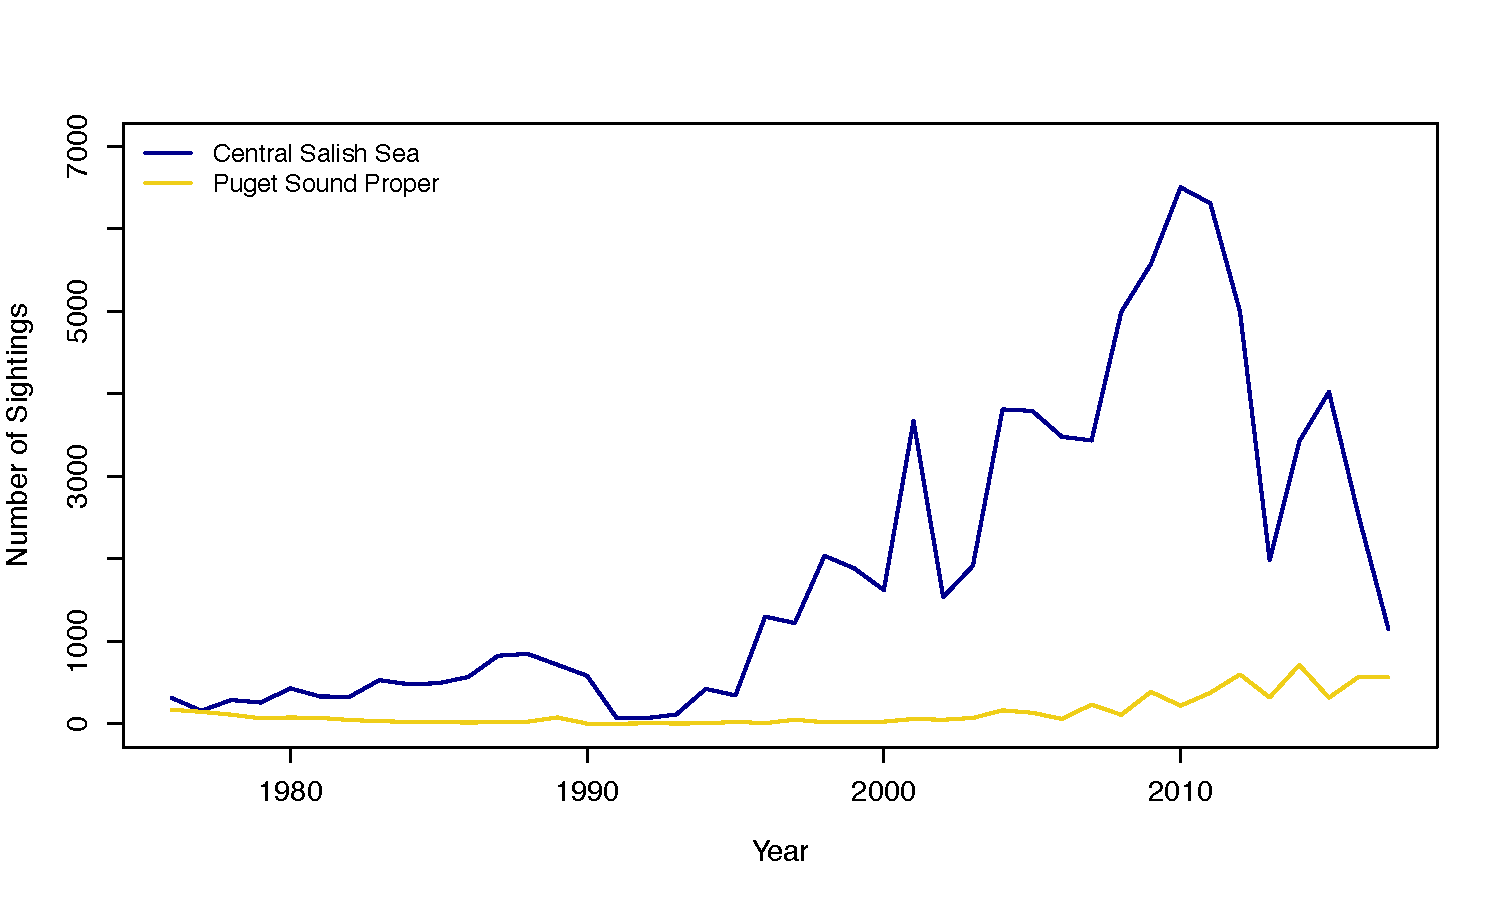
\includegraphics[width=0.8\textwidth]{../analyses/figures/OrcaPhenPlots/numsights_1976_2regs.png} 
\caption{\textbf{Sightings of SRKWs from the OrcaMaster Database}, from 1978-2017. }
\label{fig:sights}
\end{figure}

\begin{figure}[p]
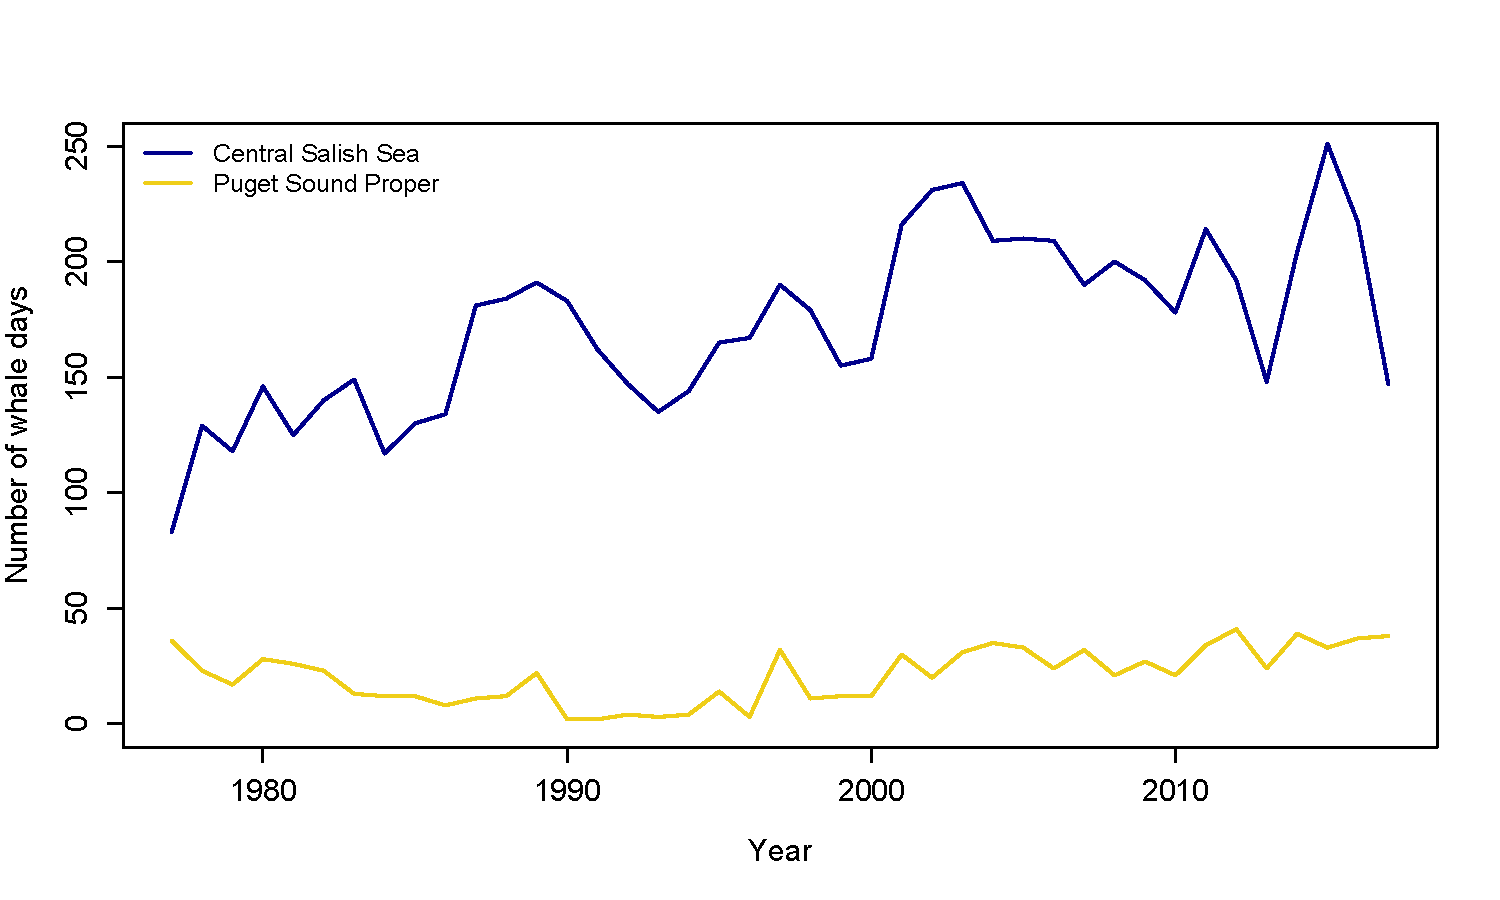
\includegraphics[width=0.8\textwidth]{../analyses/figures/OrcaPhenPlots/whaledays_assumeSRKW2regs.png} 
\caption{\textbf{Number of whale days from the OrcaMaster Database}, from 1978-2017. }
\label{fig:wdays}
\end{figure}


\begin{figure}[p]
\includegraphics[width=0.8\textwidth]{../analyses/orcaphen/figures/modwhaledays_lime.png} 
\caption{\textbf{Whale days and estimated Chinook abundance have declined at Lime Kiln State Park} since 1994. We show observed and modeled numbers of whale days from our Lime Kiln occupancy model, across all pods (A), J pod (B), K pod (C), and L pod (D), as well as estimated annual catch per unit effort (CPUE, catch per thousand fathom minutes), from our abundance model fit to Albion test fishery data from May though September across all Chinook. Shading shows 50 percentile uncertainty intervals.}
\label{fig:mlimewdays}
\end{figure}
\begin{figure}[p]
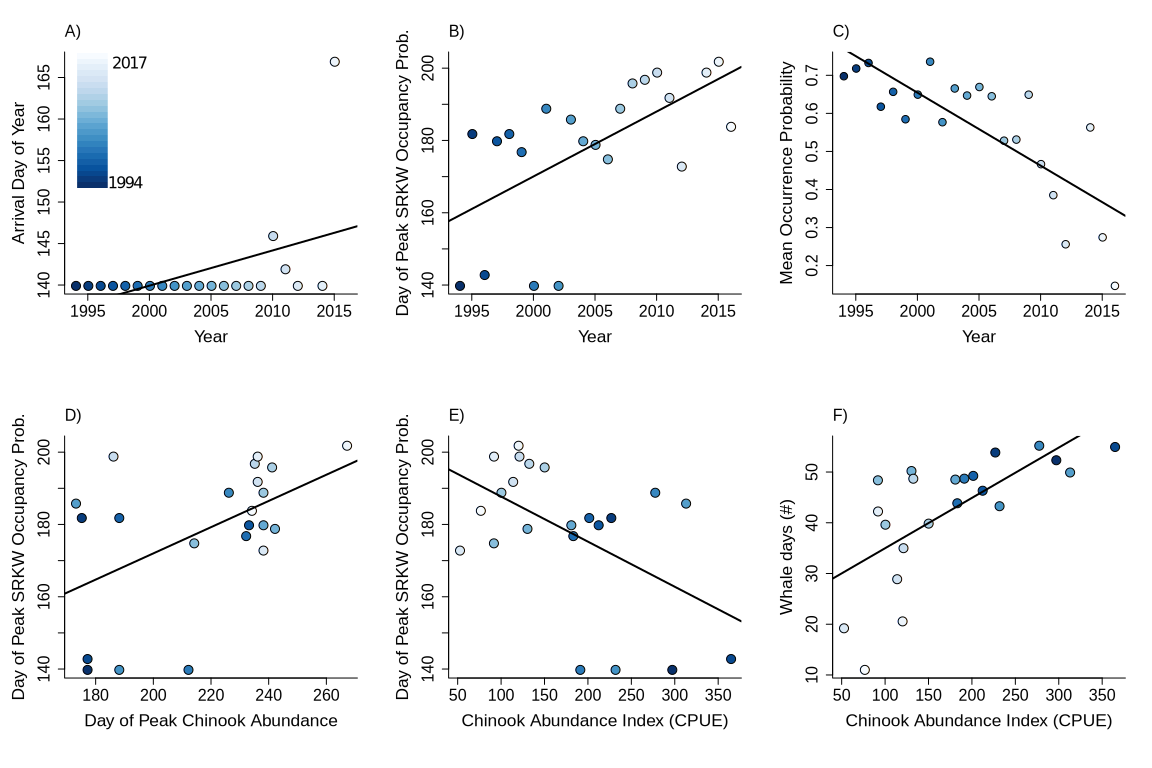
\includegraphics[width=0.8\textwidth]{../analyses/orcaphen/figures/phentrends_lime_peak.png} 
\caption{\textbf{SRKW phenology at Lime Kiln State Park is shifting}, with the likely arrival day of year (A, defined here as the first day of year when the occurrence probability is >0.20) and peak occurrence probability day of year (B) getting later, from 1994-2017. Mean occurrence probability from May to August (the season when regular monitoring of SRKWs occurs at Lime Kiln) is declining during this time period. These trends are associated with a decrease in the amount of time SRKWs are spending near Lime Kiln (i.e., the number of days on which SRKWs were observed ("whale days") has declined since 1994 (Fig. \ref{fig:mlimewdays}).}
\label{fig:limetime}
\end{figure}

\newpage
\begin{figure}[p]
\includegraphics[width=0.5\textwidth]{../analyses/orcaphen/figures/orcachinphenoverlap_allpods2006.pdf}
\caption{\textbf{SRKW phenology has shifted, in concert with shifts in Fraser River Chinook Salmon at one site with consistent observations in the Central Salish Sea}. K- and L-pod phenology (blue lines) is quantified from Lime Kiln Point State Park, SRKW phenology has shifted, with peak arrival dates delaying in recent (solid lines) compared with earlier (dashed lines) years. We show patterns for J-pod (A), K-pod (B), and L-Pod (C). Compare to Fig. 3 of the main text, which shows all pods together. }
\label{fig:KLchin}
\end{figure}

\newpage
\begin{figure}[p]
\includegraphics[width=0.9\textwidth]{../analyses/orcaphen/figures/orcachinphenoverlapSRallbrkyears.pdf}
\caption{\textbf{Changing the break-point has little qualitative effect on patterns of shifts in SRKW phenology Fraser River Chinook}. We show patterns for all SRKW pods together (as in Figure 3 in the main text) with different breakpoints of 2005 (A,B), 2006 (C,D, as in Figure 3) and 2007 (E,F). SRKW phenology (blue lines, A,C,E) is quantified from Lime Kiln Point State Park; an index of adult Fraser River Chinook salmon (summed daily CPUE from April through August, pink lines) and SRKW phenology have shifted, with peak arrival dates delaying in recent (solid lines) compared with earlier years (dashed lines).}
\label{fig:brkpt}
\end{figure}


\begin{figure}[p]
\includegraphics[width=0.8\textwidth]{../analyses/orcaphen/figures/simeffortonly2panels.png} 
\caption{\textbf{Expected change in phenology due to changes in effort alone, across Puget Sound and the Central Salish Sea regions}, from 1978-2017 (A) and from 2001-2017 (B). }
\label{fig:simeffort}
\end{figure}


\begin{figure}[p]
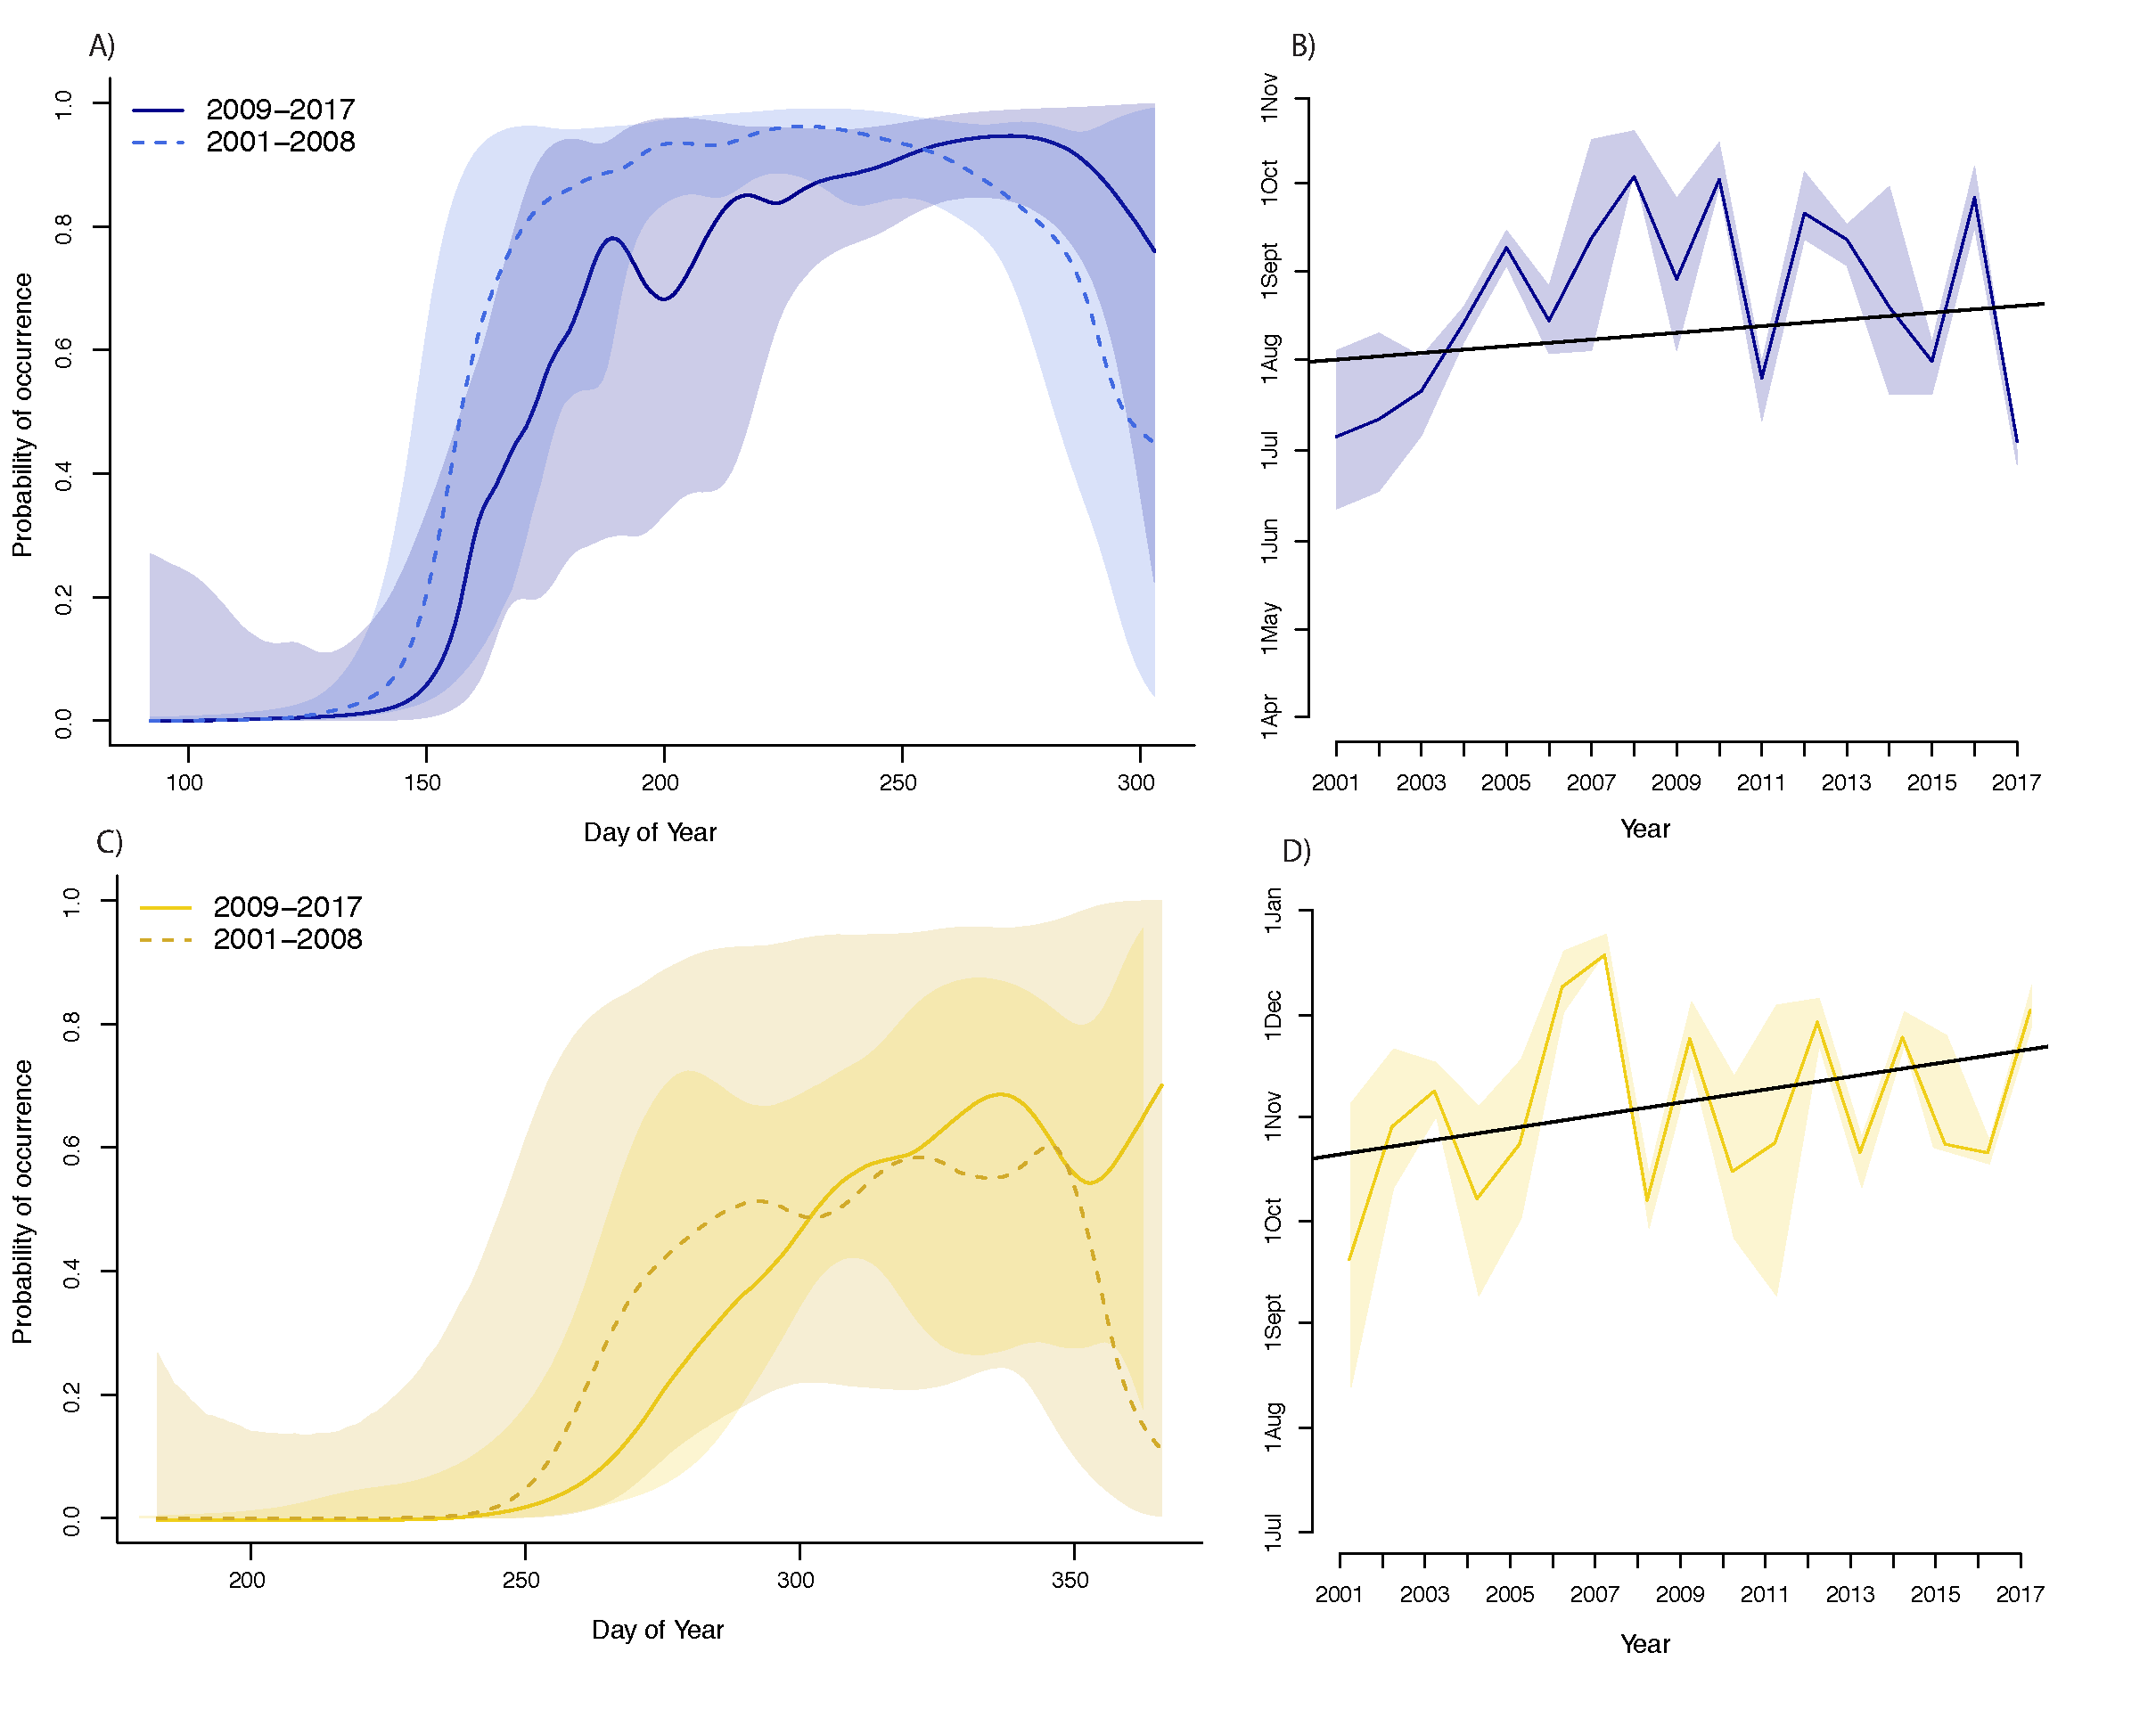
\includegraphics[width=0.8\textwidth]{../analyses/figures/proboccK_4panels.png} 
\caption{\textbf{K-pod activity varies seasonally in the Central Salish Sea (A) and Puget Sound proper (C).} This phenology has shifted later in recent years in the Central Salish Sea (B) and in Puget Sound (D). The shift toward later arrival in the central Salish Sea is evident the estimated probabilities of occurrence from the occupancy models for K-pod (A,C) as well as the linear trends in peak occurrence probability from 2001-2017 (B,D). Shading around lines represents 50\% credible intervals (95\% credible intervals in Table SX). 
}
\label{fig:Kprobs}
\end{figure}


\begin{figure}[p]
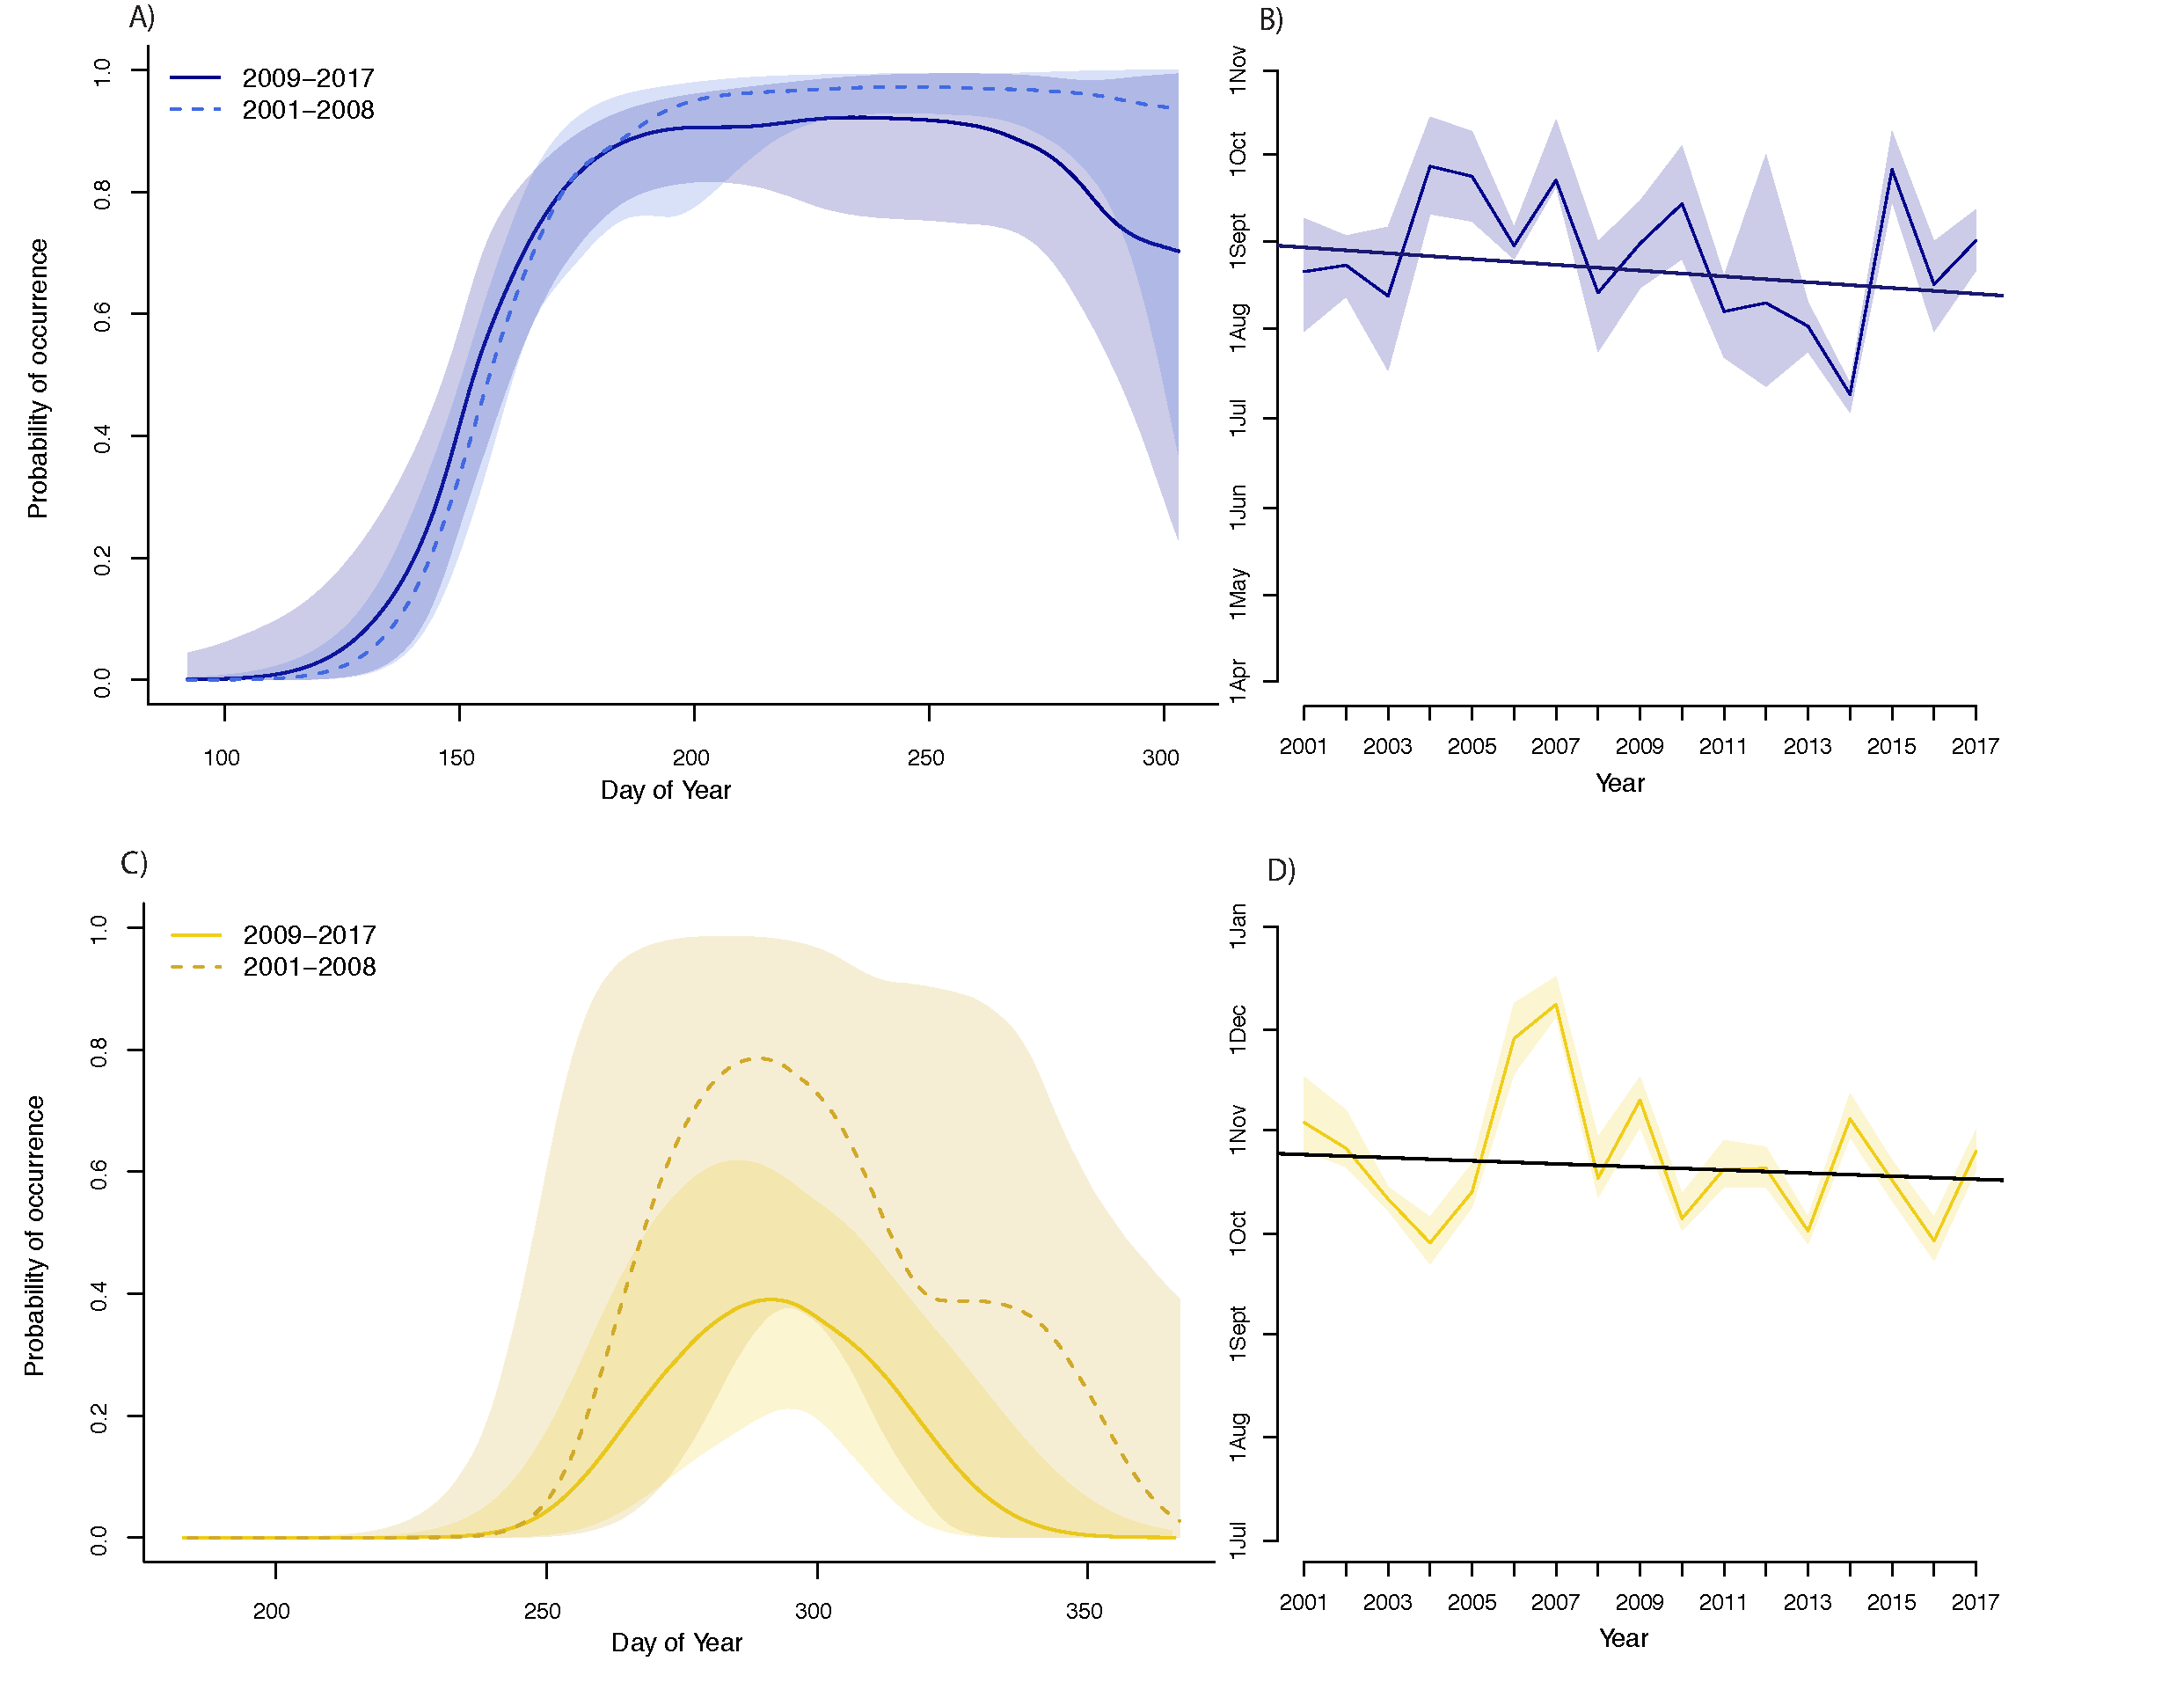
\includegraphics[width=0.8\textwidth]{../analyses/figures/proboccL_4panels.png} 
\caption{\textbf{L-pod activity varies seasonally in the Central Salish Sea (A) and Puget Sound proper (C)}. This phenology has shifted later in recent years in the Central Salish Sea (B) and in Puget Sound (D). The shift toward later arrival in the central Salish Sea is evident the estimated probabilities of occurrence from the occupancy models for K-pod (A,C) as well as the linear trends in peak occurrence probability from 2001-2017 (B,D). Shading around lines represents 50\% credible intervals (95\% credible intervals in Table SX). 
}
\label{fig:Lprobs}
\end{figure}

%Ailene’s To Do List
%Check #s and be consistent about CIs (95% in text,  50% in figures, both in supp)
%Notes for Discussion (possible points to add, from Meeting with Jameal and Chris):
%Phenology matters to killer whales in one region but not in other. Where it matters, things that modify timing should be included. Indirect to think about how hatchery timing could affect that. 
%Could reference atlantic modelling or scaling up to ecosystem level by referencing Isaac’s papers. Cite Lacey paper. On the other hand, you could regulate all the fishing and vessel traffic could still inhibit prey capture for SRKWs.
%Add a sentence for cumulative impacts on recovering prey . Try to think of other similar examples- perhaps on lands. Great barrier reef- taken one conservation action but another limiting factor in play. 
%Engage cumulative impacts, EBME literature to be broader. It's widely acknowledged %that cumulative impacts are threatening SRKWs. Timing is less often considered. %Will Satherwaite paper on salmon. Forecasting with SRKWs- managing 
%Disproportionate importance of some timing- Are there particular times of year  %when SRKWs are more sensitive to starvation (e.g. due to birth)? 
%Overall abundance is still important for prey.  But its not the whole story. %Phenology is not the whole story either.
%Fisheries are more direct way of managing prey than hatcheries.
\newpage

%%%%%%%%%%%%%%%%%%%%%%%%%%%%%%%%%%%%%%
  \end{document}
%%%%%%%%%%%%%%%%%%%%%%%%%%%%%%%%%%%%%%
